\documentclass[
	12pt,
	a4paper,
	bibtotoc,
	cleardoubleempty, 
	idxtotoc,
	ngerman,
	openright
	final,
	listof=nochaptergap,
	]{scrbook}

\usepackage[T1]{fontenc}
\usepackage[utf8]{inputenc}


\usepackage[ngerman]{babel}

% ##################################################
% Dokumentvariablen
% ##################################################

% Persoenliche Daten
\newcommand{\docNachnameEins}{Arulsothy}
\newcommand{\docVornameEins}{Sugirthan}
\newcommand{\docNachnameZwei}{Hirt}
\newcommand{\docVornameZwei}{Marius}
\newcommand{\docNachnameDrei}{Mattes}
\newcommand{\docVornameDrei}{Oliver}
\newcommand{\docNachnameVier}{Türkmen}
\newcommand{\docVornameVier}{Yasemin}

\newcommand{\docOrt}{Furtwangen}

% Dokumentdaten
\newcommand{\docTitle}{Convolutional Neural Networks}
\newcommand{\docUntertitle}{Qualitätsanalyse und Vorhersage von Komponenten des Weinschorle-Automaten}
\newcommand{\docArtDerArbeit}{Projektdokumentation}
\newcommand{\docStudiengang}{AIN/ITP}
\newcommand{\docAbgabedatum}{\today}
\newcommand{\docErsterReferent}{Prof. Dr. Christoph Reich}
\newcommand{\docZweiterReferent}{Matthias Lermer}

% ##################################################
% Allgemeine Pakete
% ##################################################

% Abbildungen einbinden
\usepackage{graphicx}

% Zusaetsliche Sonderzeichen
\usepackage{dingbat}

% Farben
\usepackage{color}
\usepackage[usenames,dvipsnames,svgnames,table]{xcolor}

% Maskierung von URLs und Dateipfaden
\usepackage[hyphens]{url}

% Deutsche Anfuehrungszeichen
\usepackage[babel, german=quotes]{csquotes}

% Pakte zur Index-Erstellung (Schlagwortverzeichnis)
\usepackage{index}
\makeindex

% ##################################################
% Seitenformatierung
% ##################################################
\usepackage[
	portrait,
	bindingoffset=1.5cm,
	inner=2.5cm,
	outer=2.5cm,
	top=3cm,
	bottom=2cm,
	%includeheadfoot
	]{geometry}

% ##################################################
% Kopf- und Fusszeile
% ##################################################

\usepackage{fancyhdr}

\pagestyle{fancy}
\fancyhf{}
\fancyhead[EL,OR]{\sffamily\thepage}
\fancyhead[ER,OL]{\sffamily\leftmark}

\fancypagestyle{headings}{}

\fancypagestyle{plain}{}

\fancypagestyle{empty}{
  \fancyhf{}
  \renewcommand{\headrulewidth}{0pt}
}

%Kein "Kapitel # NAME" in der Kopfzeile
\renewcommand{\chaptermark}[1]{
	\markboth{#1}{}
   	\markboth{\thechapter.\ #1}{}
}

% ##################################################
% Schriften
% ##################################################

% Stdandardschrift festlegen
\renewcommand{\familydefault}{\sfdefault}

% Standard Zeilenabstand: 1,5 zeilig
\usepackage{setspace}
\onehalfspacing 

% Schriftgroessen festlegen
\addtokomafont{chapter}{\sffamily\large\bfseries} 
\addtokomafont{section}{\sffamily\normalsize\bfseries} 
\addtokomafont{subsection}{\sffamily\normalsize\mdseries} 
\addtokomafont{caption}{\sffamily\normalsize\mdseries} 

% ##################################################
% Inhaltsverzeichnis / Allgemeine Verzeichniseinstellungen
% ##################################################

\usepackage{tocloft}

% Punkte auch bei Kapiteln
\renewcommand{\cftchapdotsep}{3}
\renewcommand{\cftdotsep}{3}

% Schriftart und -groesse im Inhaltsverzeichnis anpassen
\renewcommand{\cftchapfont}{\sffamily\normalsize}
\renewcommand{\cftsecfont}{\sffamily\normalsize}
\renewcommand{\cftsubsecfont}{\sffamily\normalsize}
\renewcommand{\cftchappagefont}{\sffamily\normalsize}
\renewcommand{\cftsecpagefont}{\sffamily\normalsize}
\renewcommand{\cftsubsecpagefont}{\sffamily\normalsize}

%Zeilenabstand in den Verzeichnissen einstellen
\setlength{\cftparskip}{.5\baselineskip}
\setlength{\cftbeforechapskip}{.1\baselineskip}

% ##################################################
% Abbildungsverzeichnis und Abbildungen
% ##################################################

\usepackage{caption}

\usepackage{wrapfig}

% Nummerierung von Abbildungen
\renewcommand{\thefigure}{\arabic{figure}}
\usepackage{chngcntr}
\counterwithout{figure}{chapter}

% Abbildungsverzeichnis anpassen
\renewcommand{\cftfigpresnum}{Abbildung }
\renewcommand{\cftfigaftersnum}{:}

% Breite des Nummerierungsbereiches [Abbildung 1:]
\newlength{\figureLength}
\settowidth{\figureLength}{\bfseries\cftfigpresnum\cftfigaftersnum}
\setlength{\cftfignumwidth}{\figureLength}
\setlength{\cftfigindent}{0cm}

% Schriftart anpassen
\renewcommand\cftfigfont{\sffamily}
\renewcommand\cftfigpagefont{\sffamily}


% ##################################################
% Tabellenverzeichnis und Tabellen
% ##################################################

% Nummerierung von Tabellen
\renewcommand{\thetable}{\arabic{table}}
\counterwithout{table}{chapter}

% Tabellenverzeichnis anpassen
\renewcommand{\cfttabpresnum}{Tabelle }
\renewcommand{\cfttabaftersnum}{:}

% Breite des Nummerierungsbereiches [Tabelle 1:]
\newlength{\tableLength}
\settowidth{\tableLength}{\bfseries\cfttabpresnum\cfttabaftersnum}
\setlength{\cfttabnumwidth}{\tableLength}
\setlength{\cfttabindent}{0cm}

%Schriftart anpassen
\renewcommand\cfttabfont{\sffamily}
\renewcommand\cfttabpagefont{\sffamily}

% Unterdrueckung von vertikalen Linien
\usepackage{booktabs}

% ##################################################
% Listings (Quellcode)
% ##################################################

\usepackage{listings}
\lstset{
	language=java,
	backgroundcolor=\color{white},
	breaklines=true,
	prebreak={\carriagereturn},
 	breakautoindent=true,
 	numbers=left,
 	numberstyle=\tiny,
 	stepnumber=2,
 	numbersep=5pt,
 	keywordstyle=\color{blue},
   	commentstyle=\color{green},   
   	stringstyle=\color{gray}
}
  	
% ##################################################
% Theoreme
% ##################################################
  	
% Umgebung für Beispiele
\newtheorem{beispiel}{Beispiel}

% Umgebung für These
\newtheorem{these}{These}

% Umgebung für Definitionen
\newtheorem{definition}{Definition}

% Umgebung für Formeln
\newtheorem{formel}{Formel}
  	
% ##################################################
% Literaturverzeichnis
% ##################################################

\usepackage{natbib}

% ##################################################
% Abkuerzungsverzeichnis
% ##################################################

\usepackage[printonlyused]{acronym}

% ##################################################
% PDF / Dokumenteninternelinks
% ##################################################

\usepackage[
	colorlinks=false,
   	linkcolor=black,
   	citecolor=black,
  	filecolor=black,
	urlcolor=black,
    bookmarks=true,
    bookmarksopen=true,
    bookmarksopenlevel=3,
    bookmarksnumbered,
    plainpages=false,
    pdfpagelabels=true,
    hyperfootnotes,
    pdftitle ={\docTitle},
    pdfauthor={\docVornameEins~\docNachnameEins},
    pdfcreator={\docVornameEins~\docNachnameEins}]{hyperref}

\begin{document}

\setcounter{secnumdepth}{3}

% Titelblatt
\begin{titlepage}
\pagestyle{empty}

% ##################################################
% HFU-Logo einbinden
% ##################################################
\begin{flushright}
\begin{figure}[ht]
\flushright

\includegraphics[height=3cm]{content/pictures/HFU_Logo.jpg}
\end{figure}
\end{flushright}

% ##################################################
% Titel
% ##################################################
\begin{center}
{\fontsize{18}{22} \selectfont \docArtDerArbeit}\\[5mm]
{\fontsize{18}{22} \selectfont im Studiengang} \\[5mm]
{\fontsize{18}{22} \selectfont \docStudiengang}\\
\vspace{1cm}
\begin{onehalfspace}
{\fontsize{22}{26} \selectfont \textbf{\docTitle}}\\[5mm]
{\fontsize{18}{22} \selectfont \docUntertitle}


\end{onehalfspace}
\end{center}

% ##################################################
% Zusatzinformationen
% ##################################################
\vfill
\begin{center}
\begin{tabular}{lcl}
Referent  		&:& \docErsterReferent 	\\ \\
Koreferent 		&:& \docZweiterReferent \\ \\	
Vorgelegt am 	&:& \docAbgabedatum 	\\ \\
Vorgelegt von 	&:& \docVornameEins~\docNachnameEins\\
				& & \docVornameZwei~\docNachnameZwei\\
				& & \docVornameDrei~\docNachnameDrei\\
				& & \docVornameVier~\docNachnameVier			
\end{tabular}
\end{center}
\end{titlepage}
\cleardoubleemptypage

\frontmatter
\pagenumbering{Roman}

% Abstract
\chapter*{Abstract\markboth{Abstract}{}}
\addcontentsline{toc}{chapter}{Abstract}
Im Herbst 2017 wurde als Einsendung für den Wettbewerb „CLOUD-MEISTER 2017“ der Weinschorle-Automat WISH 4.0 entwickelt. Im Rahmen des Semesterprojektes des Sommersemesters 2018 sollte dieser weiterentwickelt werden. Diese Arbeit dokumentiert die an das Weiterentwicklungsprojekt gestellten Anforderungen, sowie Umsetzung, Probleme und Ergebnisse von diesem.

Dabei haben wir uns mit drei funktionalen Anforderungen auseinandergesetzt, von denen wir sowohl die Klassifizierung verschiedener Glasformen, als auch das Feststellen von Verschmutzung des Drehtellers mithilfe von \ac{CNN} umsetzen konnten. Die Volumenberechnung von Gläsern wurde aufgrund von technischen Grenzen der Kinect nach ersten Tests nicht weiterverfolgt. 

\cleardoubleemptypage

% Inhaltsverzeichnis
\tableofcontents
\addcontentsline{toc}{chapter}{Inhaltsverzeichnis}
\cleardoubleemptypage

% Abbildungsverzeichnis einbinden und ins Inhaltsverzeichnis
\addcontentsline{toc}{chapter}{\listfigurename} 
\listoffigures
\cleardoubleemptypage

% Tabellenverzeichnis einbinden und ins Inhaltsverzeichnis
\addcontentsline{toc}{chapter}{\listtablename}
\listoftables
\cleardoubleemptypage

% Abkürzungsverzeichnis
\chapter*{Abkürzungsverzeichnis\markboth{Abkürzungsverzeichnis}{}}
\addcontentsline{toc}{chapter}{Abkürzungsverzeichnis}
\begin{acronym}
	\acro{CNN}{Convolutional Neural Network}
\end{acronym}

\mainmatter

% Inhalt der Arbeit / Kapitel
\chapter{Einleitung}
Im Rahmen des Wettbewerbes „CLOUD-MEISTER 2017: DER WAGO - IDEENWETTBEWERB“ hat ein Team von Studierenden um Herrn Reich den Weinschorle-Automaten „WISH 4.0“ entwickelt. Am Smartphone, Tablet oder Computer lässt sich dabei das gewünschte Mischverhältnis des Schorles per Webseite angeben, das eingestellte Glas wird per Webcam bemessen, das Volumen bestimmt und anschließend über mehrere Ventile das Schorle gemischt.

Außerdem kann der Automat auch Barcodes erkennen, um früher festgelegte Mischungen wieder zu erkennen. Im Zentrum der Umsetzung standen dabei die in Tabelle \ref{tab:Umsetzung_Industrie_4_0} dargestellten Industrie 4.0 Konzepte.

\begin{table}
	\caption{Umsetzung der Industrie 4.0 Konzepte im WISH 4.0}
	\label{tab:Umsetzung_Industrie_4_0}
	\begin{tabular}{p{0.5\linewidth}|p{0.5\linewidth}}
		Industrie 4.0 Konzept & WISH 4.0 Umsetzung \\
		\hline \hline
		Individualisierte Produktion & Individuelles Glas, Mischverhältnis, Füllmenge und Glas-Label \\
		\hline
		Prozessoptimierung in der Cloud & Nutzungsabhängige Auswahl des Befüllers \\
		\hline
		Zustandsüberwachung (Condition Monitoring) in der Cloud & Parameter der Befüller wird überwacht \\
		\hline
		Optimierte Wartung & Je nach Nutzung wird der Bedarf einer Wartung bestimmt \\
		\hline
		Cloud Steuerung & Meta-Steuerbefehle (z.B. fülle Glas) werden von der Cloud an die Lokale Steuerung geschickt
		Lokale Steuerung (WAGO-Controller) führt die Geräte-Befehle aus \\
		\hline
		Visual Quality Management & Visuelle Erkennung von verschiedenen Gläsern in der Cloud \\
		\hline
		Smart Logistics  & Erkennung des Barcodes, Kupplung zu Glas, und Speicherung für weitere Verarbeitung \\
		\hline
		Supply Chain Compliance & Einhaltung vordefinierter Compliance Vorgaben bezüglich des zu druckenden Labels \\
	\end{tabular}
\end{table}
\chapter{Gläser}
\section{Anforderungen und Ziele}
Der Weinschorle-Automat soll eine Vielfalt verschiedener Glasformen erkennen um vor dem Befüllen dem Glas ein vordefiniertes Volumen zuordnen können. Ziel dieser Aufgabe ist das Vertraut machen mit Python an sich und insbesondere mit dem Skript, welches bereits in der Cloud für die Zuordnung zuständig ist.

\section{Ausgangssituation}
\begin{wrapfigure}{rt}{0.6\linewidth}
	\centering
	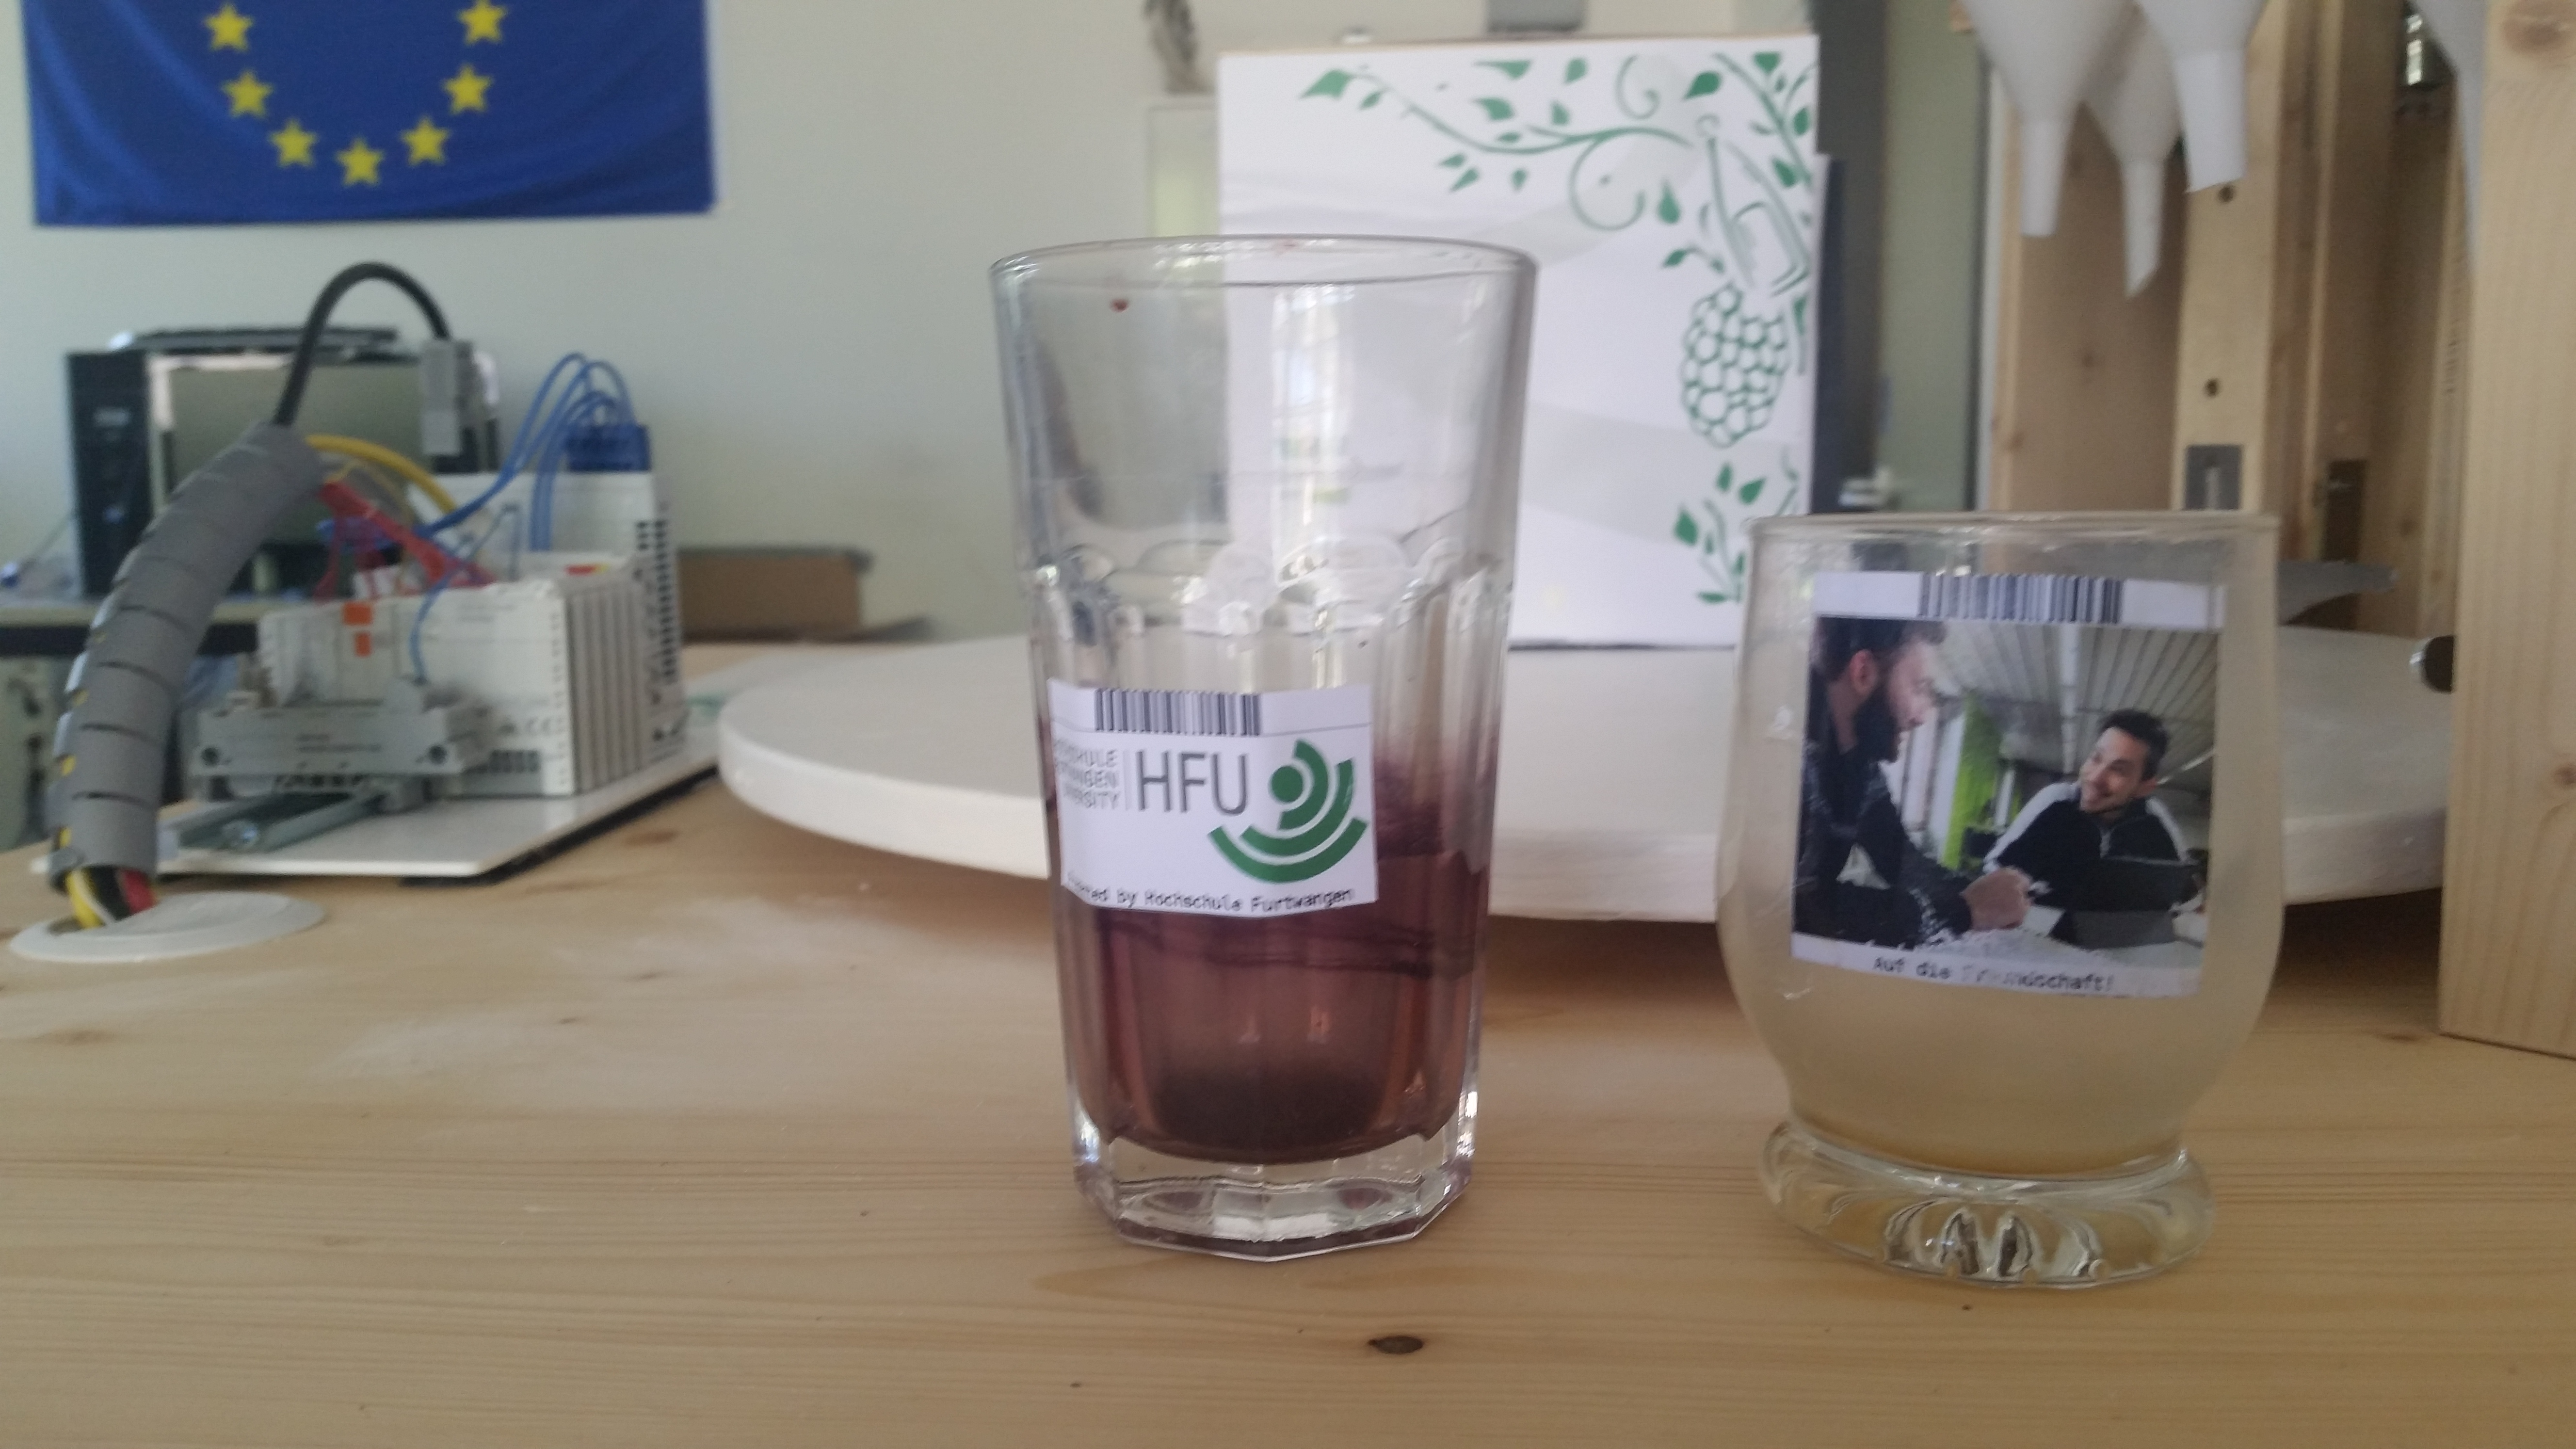
\includegraphics[width=\linewidth]{content/pictures/urspruengliche_glaeser}
	\caption{Ursprünglich bekannte Gläser}
	\label{fig:urspruengliche_glaeser}
	
	\centering
	\includegraphics[width=\linewidth]{content/pictures/position_der_kamera}
	\caption{Position der Kamera}
	\label{fig:kamera_position}
\end{wrapfigure}
Der Automat kann zu Beginn des Projekts bereits zwischen zwei unterschiedlichen Glastypen unterschieden (siehe Abbildung \ref{fig:urspruengliche_glaeser}). Dazu nimmt eine vertikal in der Fotokammer angebrachte Kamera (siehe Abbildung \ref{fig:kamera_position}) ein Bild des eingestellten Glases auf, welches zunächst zur Performance-Verbesserung auf ein kleineres Format zugeschnitten wird. Dieses Bild wird als Eingabe für das \ac{CNN} übergeben. Als Ausgabe wird das Glas im Automaten mit einer gewissen Wahrscheinlichkeit einem der beiden bekannten Glasformen zugeordnet. Basierend auf diesem Ergebnis wird die Befüll-Routine durchgeführt.
\clearpage

\section{Vorgehen}
\subsection{Trainingsdaten sammeln}
\begin{figure}[!h]
	\centering
	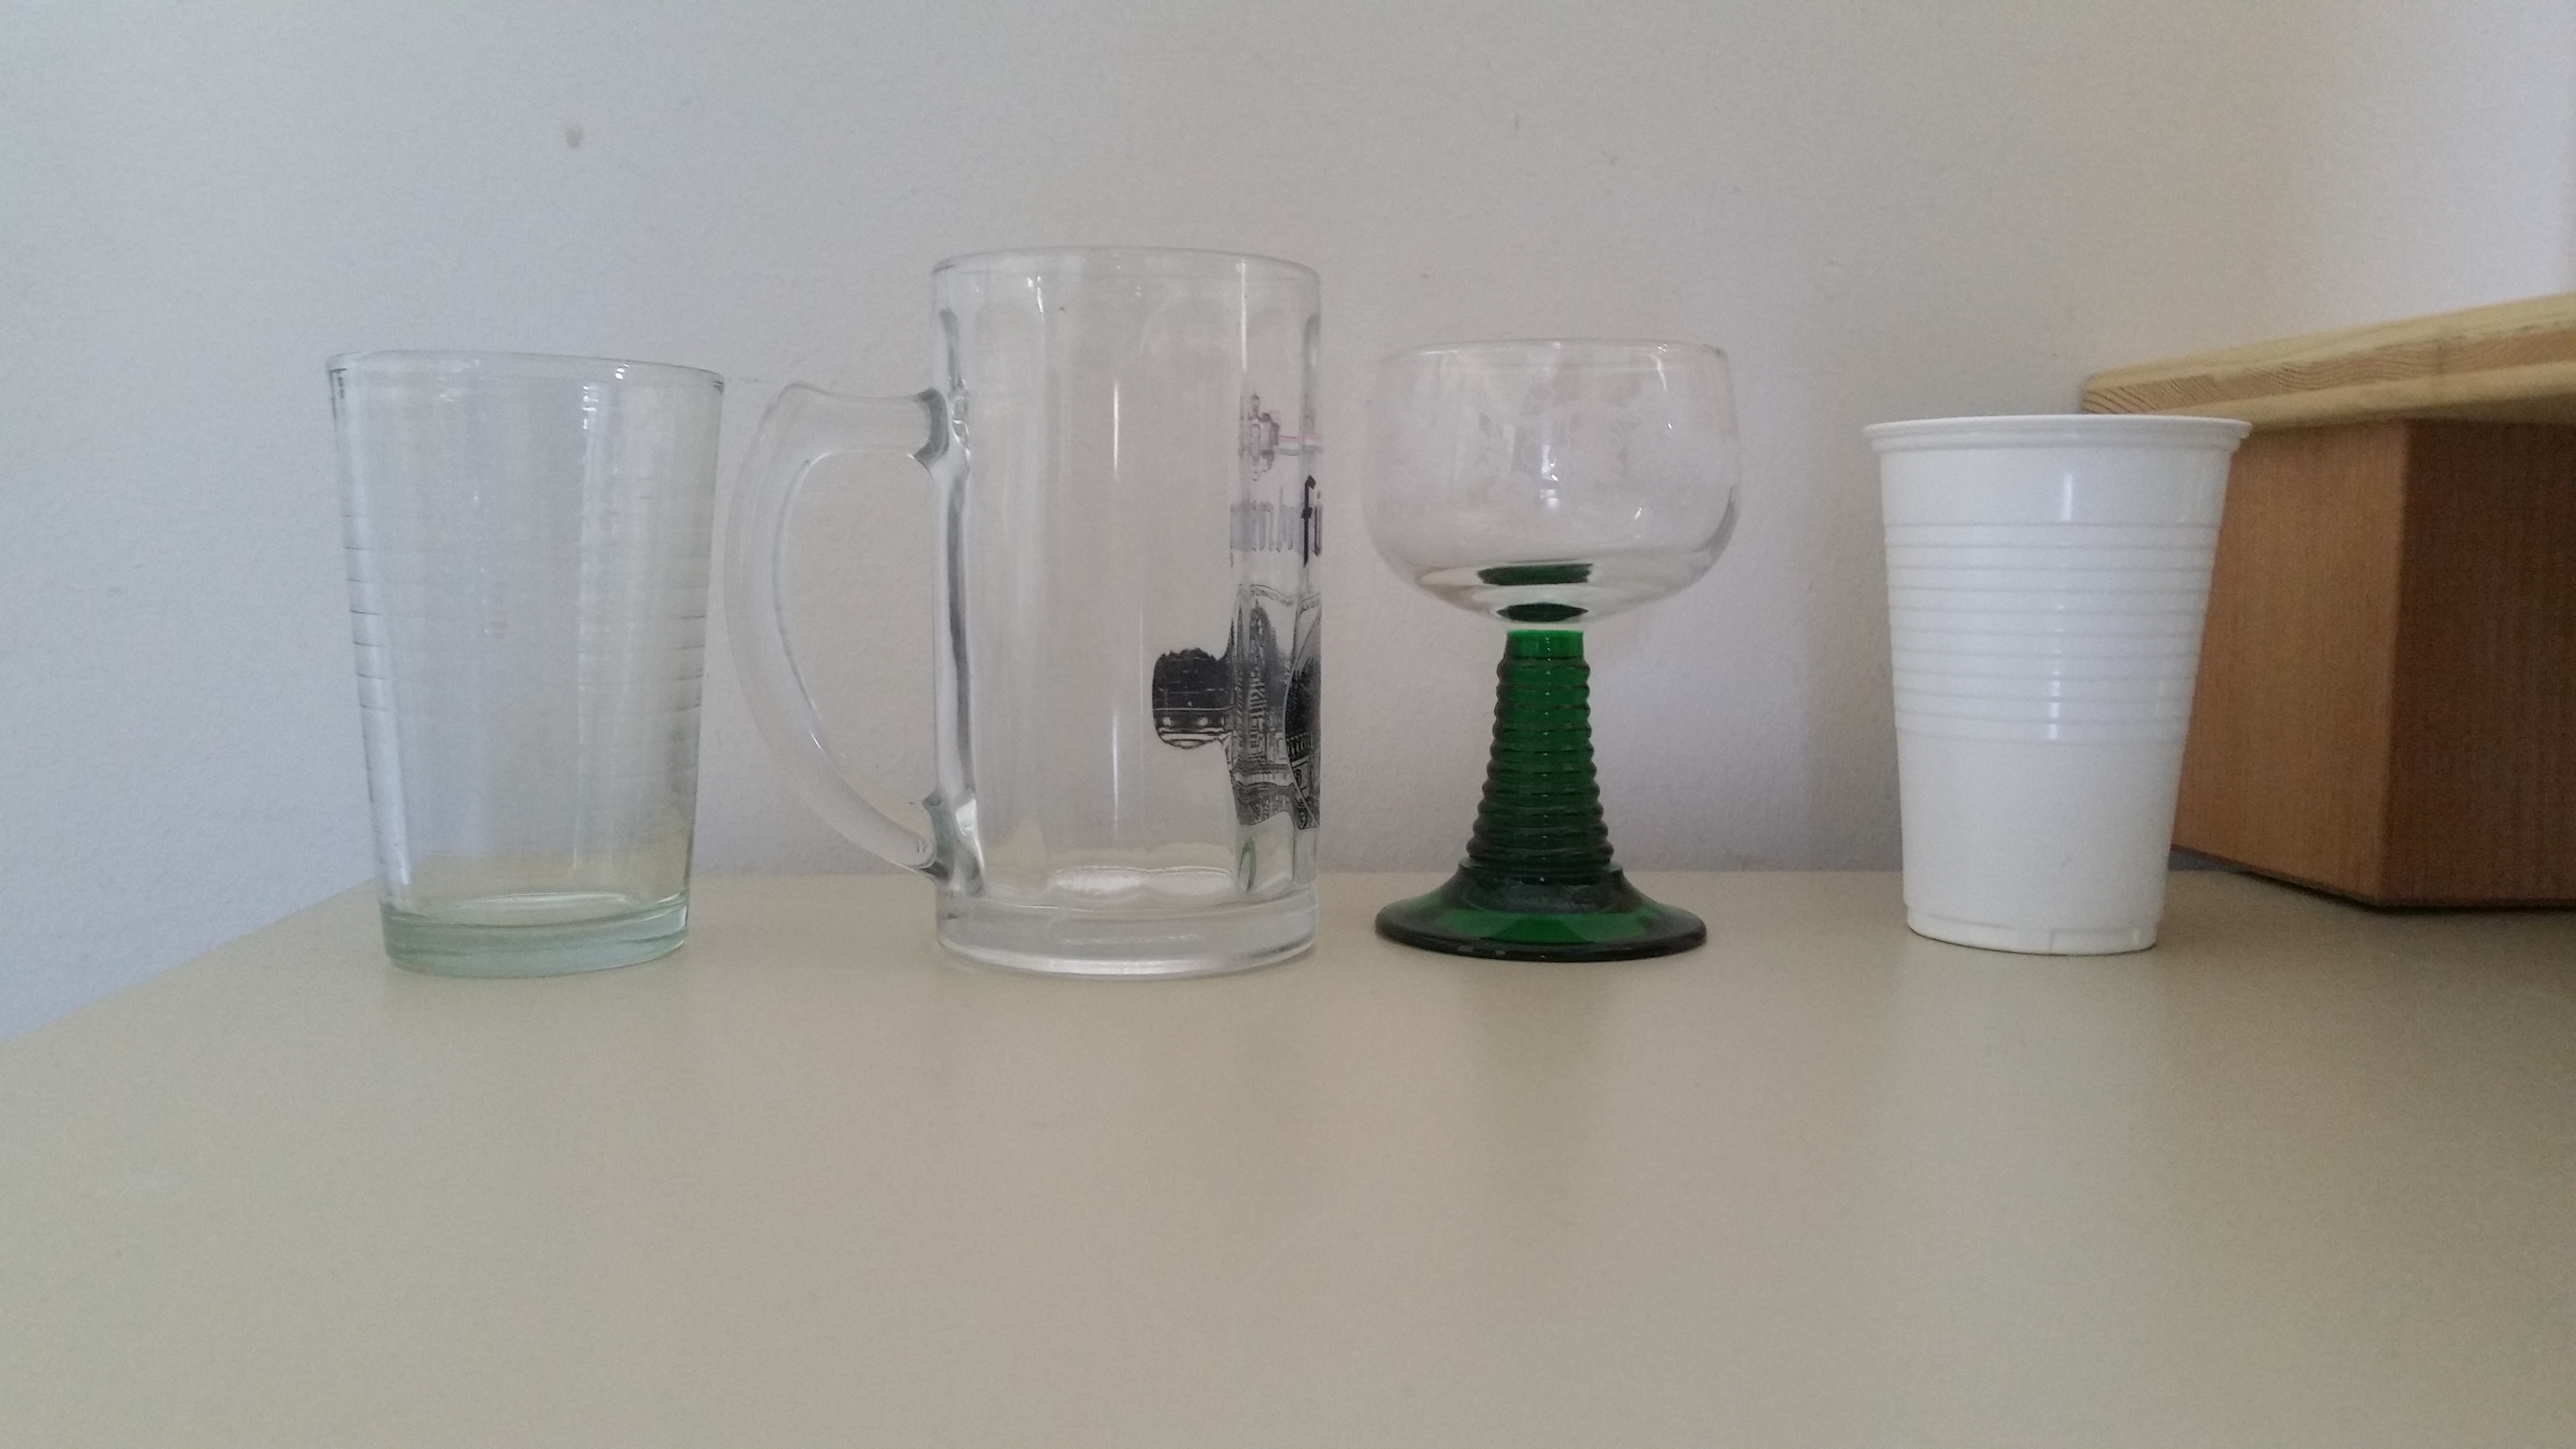
\includegraphics[width=0.7\linewidth]{content/pictures/neue_glaeser}
	\caption{Neue Gläser}
	\label{fig:neue_glaeser}
\end{figure}
Zunächst wurde die Kamera von dem Weinschorle-Automat getrennt und direkt an einen Laptop angeschlossen. Über diesen haben wir automatisch eine Serie von 100 Bildern für insgesamt vier neue Glasformen (siehe Abbildung \ref{fig:neue_glaeser}) aufgenommen. Zwischen den Aufnahmen war jeweils eine Verzögerung von drei Sekunden, so dass wir das Glas zwischen den Aufnahmen drehen konnten. Dadurch haben wir ein diverses Trainingsdatenset erzeugt, was die Trainingseffektivität des \ac{CNN} verbessert. 

\subsection{Trainingsdaten und Script anpassen}
Bevor wir das \ac{CNN} mit diesen Daten trainieren konnten mussten wir die Bilder zuschneiden (siehe Abbildung \ref{fig:vergleich_glas_zuschnitt}). Dies geschah mit dem selben Python-Script, welches bereits in der Routine des Weinschorle-Automaten verwendet wird. Weiterhin mussten wir das Trainingsscript dahingehend anpassen, dass wir die neuen Trainingsdaten als solche deklarieren und jedem Trainingsset ein entsprechendes Label zuordnen.

Damit hat sich die Anzahl der klassifizierbaren Gläser auf insgesamt sechs erhöht. Deshalb mussten wir im Predict-Script die Dimension des Output-Tensors an die neue Anzahl der Klassen entsprechend anpassen.

\begin{figure}[!h]
	\centering
	\fbox{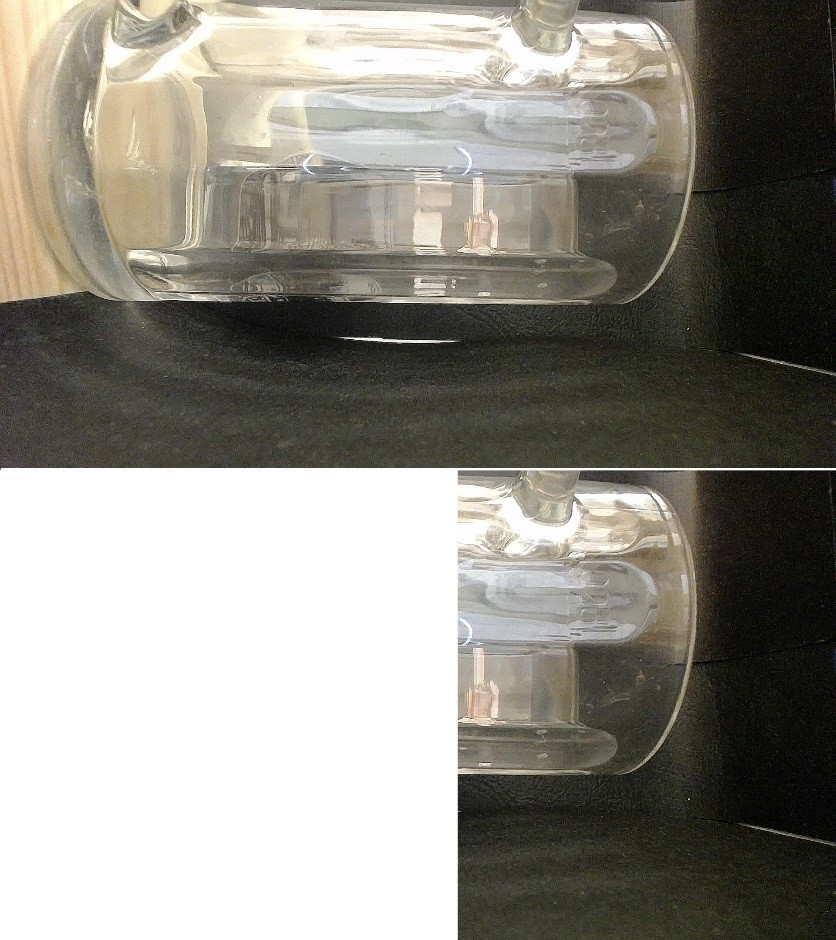
\includegraphics[width=0.7\linewidth,angle=90]{content/pictures/vergleich_glas_zuschnitt}}
	\caption{Foto vor (a) und nach (b) dem Zuschneiden}
	\label{fig:vergleich_glas_zuschnitt}
\end{figure}
\clearpage

\subsection{\ac{CNN}-Architektur}
Als Eingabe für das \ac{CNN} verwenden wir ein 3 Channel 128x128 Bild. 
Für die convolution Operationen setzen wir drei convolutional layer ein, wobei die ersten beiden aus 32 und die dritte layer aus 64 Filtern besteht. 
Dabei werden gängige 3*3 Filter verwendet.

Die tatsächliche Erkennung der Gläser übernehmen zwei FC-layer, die erste mit 128 Neuronen, die zweite mit 6 an die Anzahl der Gläser angepasst. Daraus ergibt sich die in Abbildung \ref{fig:glass_structure} gezeigte Struktur des \ac{CNN}

\begin{figure}[!h]
	\centering
	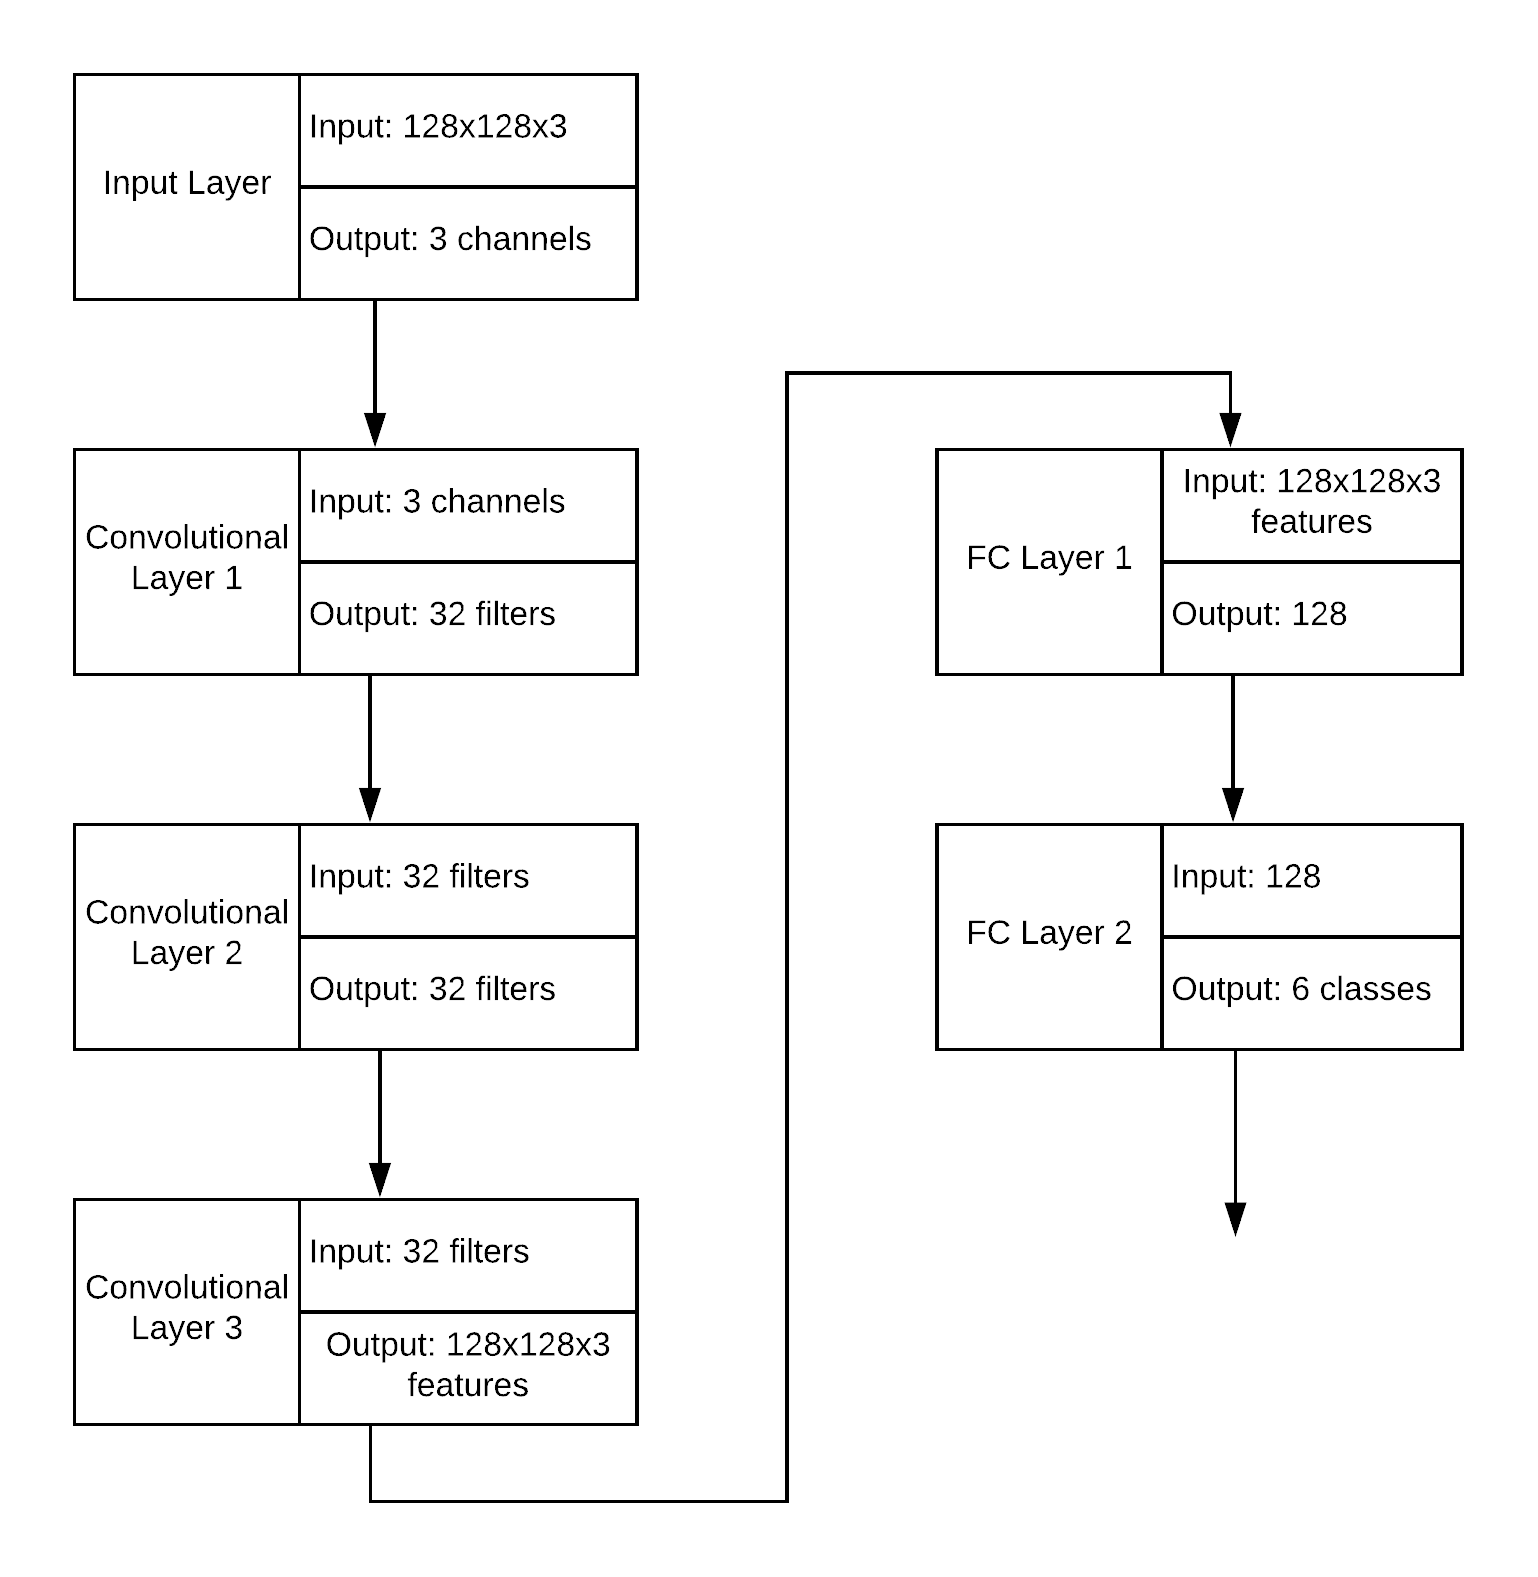
\includegraphics[width=0.7\linewidth]{content/pictures/glass_structure}
	\caption{Struktur des \ac{CNN} zur Glaserkennung}
	\label{fig:glass_structure}
\end{figure}

\chapter{Volumenberechnung mit der Kinect}
\section{Anforderungen und Ziele}
Um sich nicht mehr auf die Klassifizierung verschiedener Vordefinierter Gläsertypen verlassen zu müssen, soll der Weinschorle-Automat in der Lage sein das Volumen eines Glases mithilfe des Tiefensensors einer Microsoft Kinect zu berechnen.

\section{Vorgehen}
\subsection{Limitationen der Kinect}
Bevor wir die Kinect in den Weinschorle-Automaten einbezogen haben, testeten wir deren Möglichkeiten. Nach der Installation von notwendiger Treiber-Software begannen wir mit den Verschiedenen Modi der Kinect zu experimentieren.

Nach ersten Tests und Recherchen mussten wir feststellen, dass der Tiefensensor der Kinect bei Objekten näher als ca. 50cm keine zuverlässigen Werte liefern kann. Diese Tatsache schränkte die Positionierungsmöglichkeiten am Weinschorle-Automaten deutlich ein. Übrig blieben die beiden Möglichkeiten: 
\begin{enumerate}
	\item Vogelperspektive
	\item Frontalperspektive
\end{enumerate}

\subsection{Vogelperspektive}
Unsere erste Idee war es die Gläser von direkt über ihnen aufzunehmen. Dazu müssten wir allerdings einen Überbau konstruieren, um die Kinect mindestens 50cm über den Glasrändern anbringen zu können. (Abbildung \ref{fig:position_zur_vogelperspektive})
\begin{figure}
	\centering
	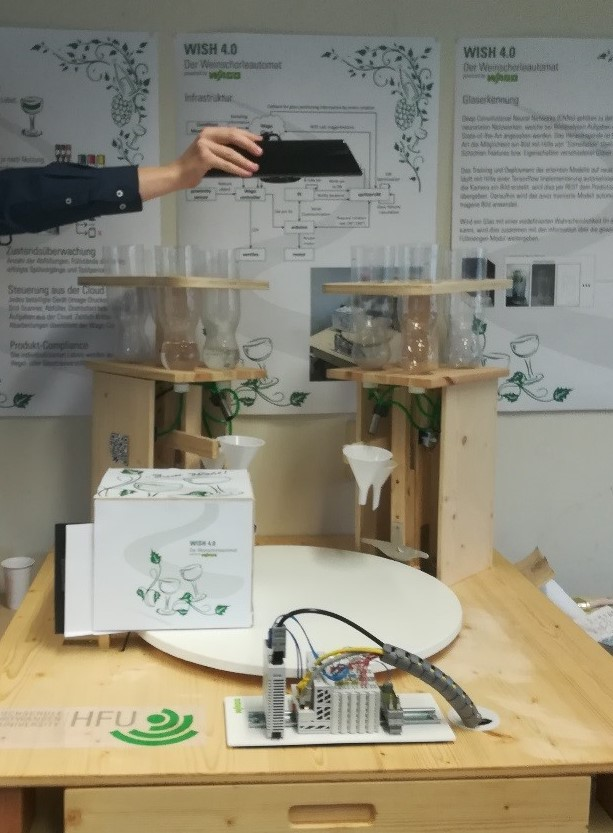
\includegraphics[width=0.5\linewidth]{content/pictures/position_zur_Vogelperspektive}
	\caption{Platzierung der Kinect für Vogelperspektive}
	\label{fig:position_zur_vogelperspektive}
\end{figure}
Vorteile dieser Positionierung sind zum einen die einfachere Messung des Volumens, da wir nur zwei Messpunkte im selben Bild benötigen. Einen für die Entfernung des Randes und einen für die Entfernung des Glasbodens zur Kinect. Daraus lässt sich dann einfach die Füllhöhe als Differenz der beiden werte berechnen. Mithilfe des Radius könnten wir das Volumen des Glases abschätzen. 

Zum andern könnten wir bei dieser Positionierung die RGB-Kamera der Kinect einsetzen, um beispielsweise die Sauberkeit des Drehtellers zu überprüfen (siehe Verschmutzung des Drehtellers).

Ein Nachteil wäre der zusätzliche Aufwand einen Überbau zu konstruieren, an dem wir die Kinect befestigen können. Außerdem muss bei diesem Ansatz das Glas zwischen den beiden Trichtern des Weinschorle-Automaten vermessen werden (siehe Abbildung \ref{fig:aufnahme_vogel}a). Dies würde uns dazu zwingen den Drehteller nach der Vermessung gegen den Uhrzeigersinn zu drehen. Da zu diesem Zeitpunkt bereits ein neues Glas auf dem Drehteller stehen könnte, würde dessen Füllroutine behindert. 

Zum Scheitern dieses Ansatzes führte schließlich die Untauglichkeit der Kinect für die Messung des Glasrandes, wie man in Abbildung \ref{fig:aufnahme_vogel}b erkennen kann. Im besten Fall sollte man an der Stelle des Glasrandes einen dunkel-grauen Ring erkennen können. Jedoch nimmt die Kinect nur undefinierte Werte auf (repräsentiert durch weiß im Bild) Die Kinect gibt Tiefenwerte von 0 (schwarz) bis 2048(weiß) für jeden Pixel in ihrem Tiefenbild an. 

\clearpage
\begin{figure}
	\centering
	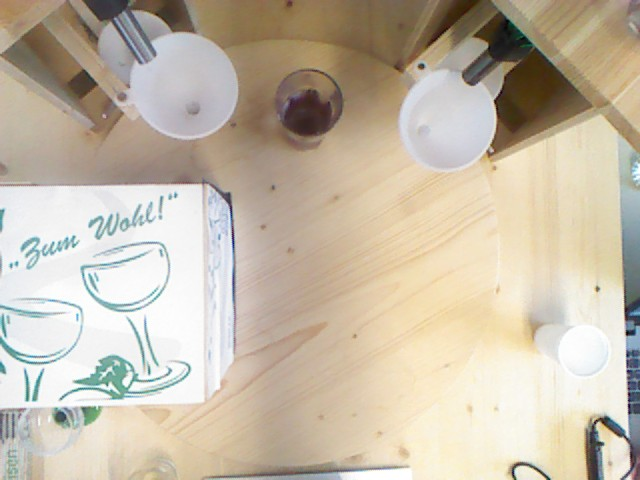
\includegraphics[width=0.45\linewidth]{content/pictures/vogel_rgb}
	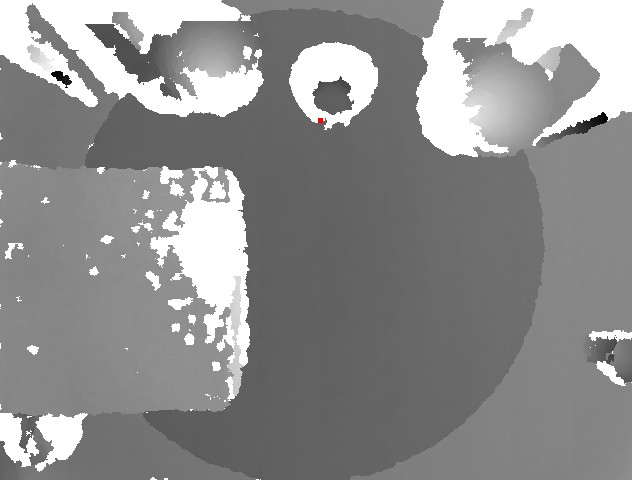
\includegraphics[width=0.45\linewidth]{content/pictures/vogel_depth}
	\caption{Kinect Aufnahme aus Vogelperspektive, RGB-Modus links (a), Tiefen-Modus rechts (b)}
	\label{fig:aufnahme_vogel}
\end{figure}

\subsection{Frontalperspektive}
Alternativ bliebe noch die Möglichkeit die Gläser frontal aufzunehmen, während sie unter dem ersten Trichter auf das Befüllen warten (siehe Abbildung \ref{fig:position_zur_frontalperspektive}a). Dazu positionieren wir die Kinect in der vorderen rechten Ecke des Tisches (siehe Abbildung \ref{fig:position_zur_frontalperspektive}b).
Aus dieser Positionierung ergeben sich folgende Vorteile:
\begin{itemize}
	\item Kein Überbau benötigt
	\item Keine Rotation des Drehtellers gegen den Uhrzeigersinn
\end{itemize}
Die Untauglichkeit der Kinect zuverlässige Werte zu liefern führt auch hier, ähnlich wie bei der Vogelperspektive, zum Scheitern des Ansatzes.

\begin{figure}[!h]
	\centering
	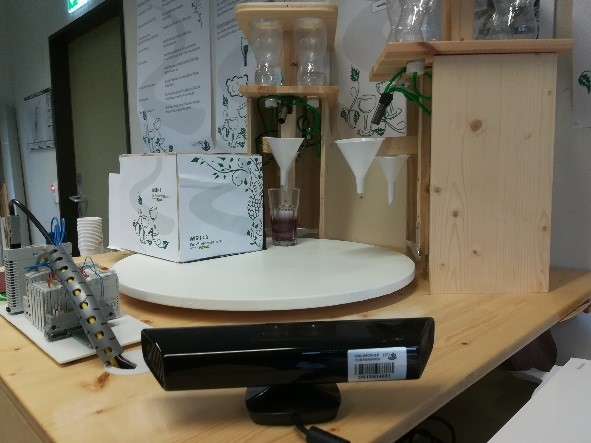
\includegraphics[width=0.45\linewidth]{content/pictures/position_zur_Frontalperspektive_behind}
	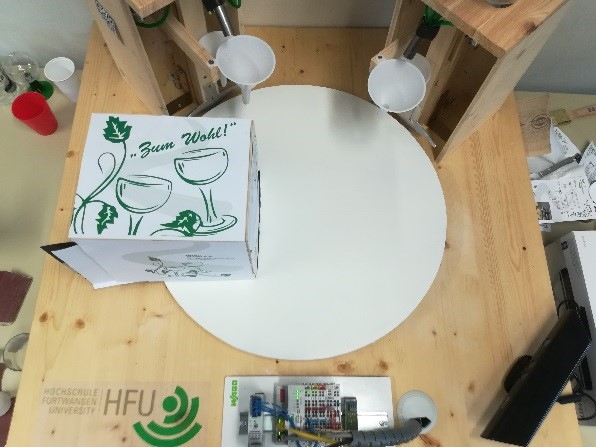
\includegraphics[width=0.45\linewidth]{content/pictures/position_zur_Frontalperspektive_top}
	\caption{Platzierung der Kinect für Frontalpositionierung}
	\label{fig:position_zur_frontalperspektive}
\end{figure}

\section{Fazit zur Kinect}
Die Kinect eignet sich nicht für Distanzen unter 50cm Entfernung, was schwer mit den Dimensionen des Weinschorle-Automaten zu vereinbaren ist. (z.B. mit einem Überbau). 

Weiterhin reicht die Auflösung der Tiefenkamera nicht aus um schmale Flächen wie einen Glas- oder Becherrand zu erfassen, was zum Scheitern unserer ersten Idee führte. 

Zuletzt scheitert diese Idee an der Tatsache, dass die Tiefenkamera der Kinect durch Projektionen von Infrarotlicht funktioniert, wobei aus den Reflektionen der Objekte ein Tiefenbild generiert wird. Durch fehlende Fähigkeit von Glas Licht zu reflektieren, ist es nahezu unmöglich dieses zu vermessen. 

Zusammenfassend genügen die Fähigkeiten der Kinect nicht den Anforderungen des Projektes.

\chapter{Verschmutzung des Drehtellers}
\section{Anforderungen und Ziele}
In Regelmäßigen Abständen soll der Verschmutzungsgrad des Drehtellers von einer Kamera erfasst und ausgewertet werden. Dabei sollen alle anstehenden und laufenden Befüll-Routinen angehalten werden, bis eine entsprechende Säuberung durchgeführt wurde.

\section{Vorgehen}
Um mögliche Komplikationen zu minimieren führen wir die Schmutzerkennung direkt vor jeder Befüll-Routine durch. Dabei ist die Kamera auf die Endposition der Gläser ausgerichtet.

Grund dafür ist die erhöhte Wahrscheinlichkeit, dass man den Inhalt des Glases beim Entnehmen verschüttet, weshalb die größte Verschmutzungsdichte eben dort zu erwarten ist. 

Vorteil davon ist, dass wir ebenfalls im Blick haben, ob das fertig befüllte Glas der vorherigen Routine beim Start einer neuen eventuell noch nicht entnommen wurde. Dies hätte zur Folge, dass ein volles Glas mit der Fotokammer kollidiert, was natürlich unerwünscht ist.

\subsection{Positionierung der Kamera}
\begin{wrapfigure}{rt}{0.6\linewidth}
	\centering
	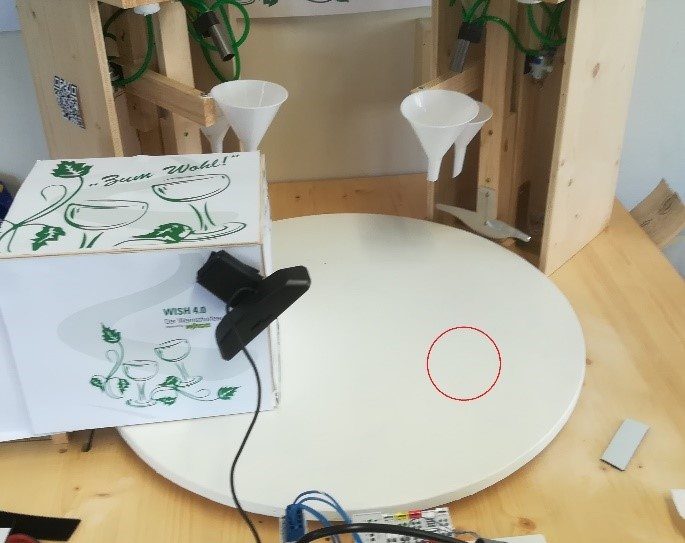
\includegraphics[width=\linewidth]{content/pictures/position_der_Kamera_zu_Schmutz}
	\caption{Positionierung der Kamera zur Schmutzerkennung}
	\label{fig:position_der_kamera_zu_schmutz}
\end{wrapfigure}
Um den Endbereich der Routine (Abbildung \ref{fig:position_der_kamera_zu_schmutz}, rechts), optimal zu Erfassen bringen wir die Kamera an der Seite der Fotokammer an (Abbildung \ref{fig:position_der_kamera_zu_schmutz}, links). Durch diese Positionierung haben wir alle relevanten Bereiche im Blick, während wir den Hintergrund minimieren.

\subsection{Trainingsdaten sammeln}
Für diesen Anwendungsfall definieren wir 3 Klassen:
\begin{itemize}
	\item Sauber
	\item Verschmutzt
	\item Besetzt
\end{itemize}
Dazu haben wir zunächst für 6 unterschiedliche Gläser jeweils 50 Bilder auf-genommen, auf welchen die Gläser an der erwarteten Endposition stehen. Diese klassifizieren wir als „besetzt“ (Abbildung \ref{fig:trainingsdaten_schmutz}c).

Als zweites haben wir insgesamt 50 Fotos des sauberen Drehtellers in verschiedenen Positionen aufgenommen und diese als „sauber“ klassifiziert (Abbildung \ref{fig:trainingsdaten_schmutz}a).

Zum Schluss haben wir mit Weiß-, Rosé-, und Rotwein jeweils 50 Bilder auf-genommen, indem wir ein Glas befüllten und den Inhalt beim Aufnehmen verschütteten, wie es auch in Anwendung sehr wahrscheinlich passieren wird. Dieses Set klassifizieren wir als „verschmutzt“ (Abbildung \ref{fig:trainingsdaten_schmutz}b, Verschmutzung oben zu erkennen).

\begin{figure}[!h]
	\centering
	
\includegraphics[width=0.25\linewidth,angle=-90]{content/pictures/2}
	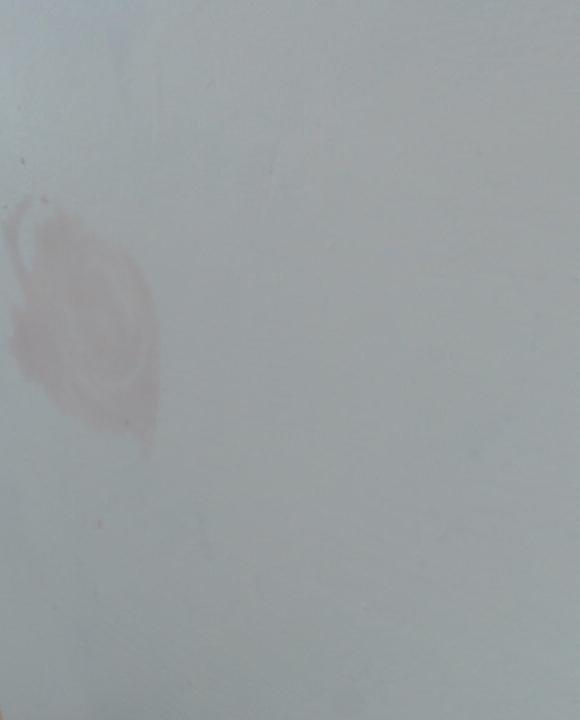
\includegraphics[width=0.25\linewidth,angle=-90]{content/pictures/1}
	
\includegraphics[width=0.25\linewidth,angle=-90]{content/pictures/0}
	\caption{Auszug aus den zugeschnittenen Trainingsdaten zur Verschmutzungserkennung (a) sauber, (b) verschmutzt und (c) besetzt}
	\label{fig:trainingsdaten_schmutz}
\end{figure}

\chapter{Fazit}
Das Projekt ist abgeschlossen, ist aufgrund der nicht implementierten Volumenberechnung als funktionale Anforderung als kritisch einzustufen.

Bezogen auf unsere Planung waren unsere Arbeitspakete unproblematisch, da diese unabhängig voneinander waren, weshalb unser kritischer Pfad wesentlich kürzer als die vorgesehene Projektdauer war. Diese haben wir je-doch voll ausnutzen müssen, da wir zum parallel an verschiedenen Anforderungen nicht genug Teilnehmer waren.

\section{Ausblick}
Angesichts der in unserem Projekt nicht erfüllten funktionalen Anforderung, die Volumenberechnung der Gläser, wäre eine Weiterentwicklung des Automaten in dieser Richtung durchaus denkbar. Da sich die Kinect aus oben genannten Bedingungen dazu jedoch nicht eignet, müsste man sich auf diesem Gebiet nach passenderen Technologien umsehen.

Weiterhin könnte man sich mit der Analyse weiterer Komponenten beschäftigen, wie zum Beispiel mit dem Füllstand der Silos. Dazu könnte man die Befülltürme für einen Überbau vorbereiten (Obere Plattformen aktuell noch lo-se). Dies würde neue Möglichkeiten zur Analyse des Zustandes vom Automaten bieten, man könnte zum Beispiel den kompletten Drehteller überwachen, und nicht nur die Entnahmeposition der Gläser, wie es aktuell implementiert ist.

Eine weitere praktische Ergänzung wäre ein direkt im Automaten integrierter Label-Drucker, welcher nach Abschluss einer Bestellung in der Webanwendung direkt das zugehörige Label bereitstellt.

Auf Software-Ebene wäre wichtig das Frontend (die Webanwendung) an die neue Routine anzupassen. Mit der Erkennung des Verschmutzungsgrades haben wir einen neuen möglichen Zustand definiert, der vom Automaten ein-genommen werden kann, welcher auf der Status-Seite der Webanwendung jedoch noch nicht berücksichtigt wird. Die gilt auch für eventuelle andere Weiterentwicklungen, wie bereits oben angemerkt.


% Schalgwortverzeichnis (Index)
\printindex

% Eidesstattliche Erklärung
\chapter*{Eidesstattliche Erklärung\markboth{Eidesstattliche Erklärung}{}} 
\addcontentsline{toc}{chapter}{Eidesstattliche Erklärung}

Ich versichere, dass ich die vorstehende Arbeit selbständig verfasst und hierzu
keine anderen als die angegebenen Hilfsmittel verwendet habe. Alle Stellen der Arbeit die 
wörtlich oder sinngemäß aus fremden Quellen entnommen wurden, sind als solche kenntlich gemacht.
\\
\\
Die Arbeit wurde bisher in gleicher oder ähnlicher Form in keinem anderen
Studiengang als Prüfungsleistung vorgelegt oder an anderer Stelle
veröffentlicht.
\\
\\
Ich bin mir bewusst, dass eine falsche Erklärung rechtliche Folgen haben kann.

\vspace*{1.5cm} \par
\line(1,0){275} \par
\docOrt, den  \docAbgabedatum ~~\docVornameEins~\docNachnameEins

\vspace*{1.5cm} \par
\line(1,0){275} \par
\docOrt, den  \docAbgabedatum ~~\docVornameZwei~\docNachnameZwei

\vspace*{1.5cm} \par
\line(1,0){275} \par
\docOrt, den  \docAbgabedatum ~~\docVornameDrei~\docNachnameDrei

\vspace*{1.5cm} \par
\line(1,0){275} \par
\docOrt, den  \docAbgabedatum ~~\docVornameVier~\docNachnameVier

\end{document}      